\documentclass{article}
\RequirePackage{amssymb}
\RequirePackage{amsmath}
\usepackage{graphicx}
\usepackage[latin1]{inputenc}

\title{Esercizio 6}
\author{Davide Angelocola}

\begin{document}
\maketitle

\section{Esercizio}
Tre libri sono messi uno sopra l'altro a formare una pila. In ogni istante se ne sceglie a caso uno e si mette in cima alla pila lasciando invariata la posizione degli altri due. Assumendo che i libri siano contraddistinti con le lettere A, B e C: descrivere con una catena di Markov il sistema il stato � costituito in ogni istante dalla disposizione dei libri nella pila.

\section{Svolgimento}

Assumendo che la pila di libri sia inizialmente cos� composta:

$$
S_1 = \begin{pmatrix} 
A \cr 
B \cr
C \cr 
\end{pmatrix}
$$

Prendendo in fondo e ponendolo in cima alla pila, ovvero prendendo il libro C e mettendolo sopra A, si ottiene la seguente pila:

$$
S_2 = \begin{pmatrix} 
C \cr 
A \cr
B \cr 
\end{pmatrix}
$$

Pescando invece il libro B si ottiene una terza pila:

$$
S_3 = \begin{pmatrix} 
B \cr 
A \cr 
C \cr
\end{pmatrix}
$$

Ripetendo questo ragionamento con B e C in cima alla pila risulta evidente che  si hanno altre 2 configurazioni con B in cima e altre 2 per C. In totale si hanno 6 \footnote{ovvero $3!$ permutazioni semplici senza ripetizioni di 3 oggetti} possibili configurazioni. Le altre tre configurazioni sono:

$$
S_4 = \begin{pmatrix} 
C \cr 
B \cr 
A \cr
\end{pmatrix}
S_5 = \begin{pmatrix} 
B \cr 
C \cr 
A \cr
\end{pmatrix}
S_6 = \begin{pmatrix} 
A \cr 
C \cr 
B \cr
\end{pmatrix}
$$

Assegnando a ciascuna configurazione uno stato possiamo quindi esibire la matrice di transizione di questa Catena di Markov, con gli stati:

$$
P = \begin{pmatrix}
\frac{1}{3} & \frac{1}{3} & \frac{1}{3} & 0 & 0 & 0 \cr 
0 & \frac{1}{3} & 0 & 0 & \frac{1}{3} & \frac{1}{3} \cr 
\frac{1}{3} & 0 & \frac{1}{3} & \frac{1}{3} & 0 & 0 \cr 
0 & 0 & 0 & \frac{1}{3} & \frac{1}{3} & \frac{1}{3} \cr 
0 & 0 & \frac{1}{3} & \frac{1}{3} & \frac{1}{3} & 0 \cr 
0 & \frac{1}{3} & \frac{1}{3} & 0 & 0 & \frac{1}{3} \cr  
\end{pmatrix}
$$

e la relativa rappresentazione con il grafo:

\begin{figure}[h]
\centering
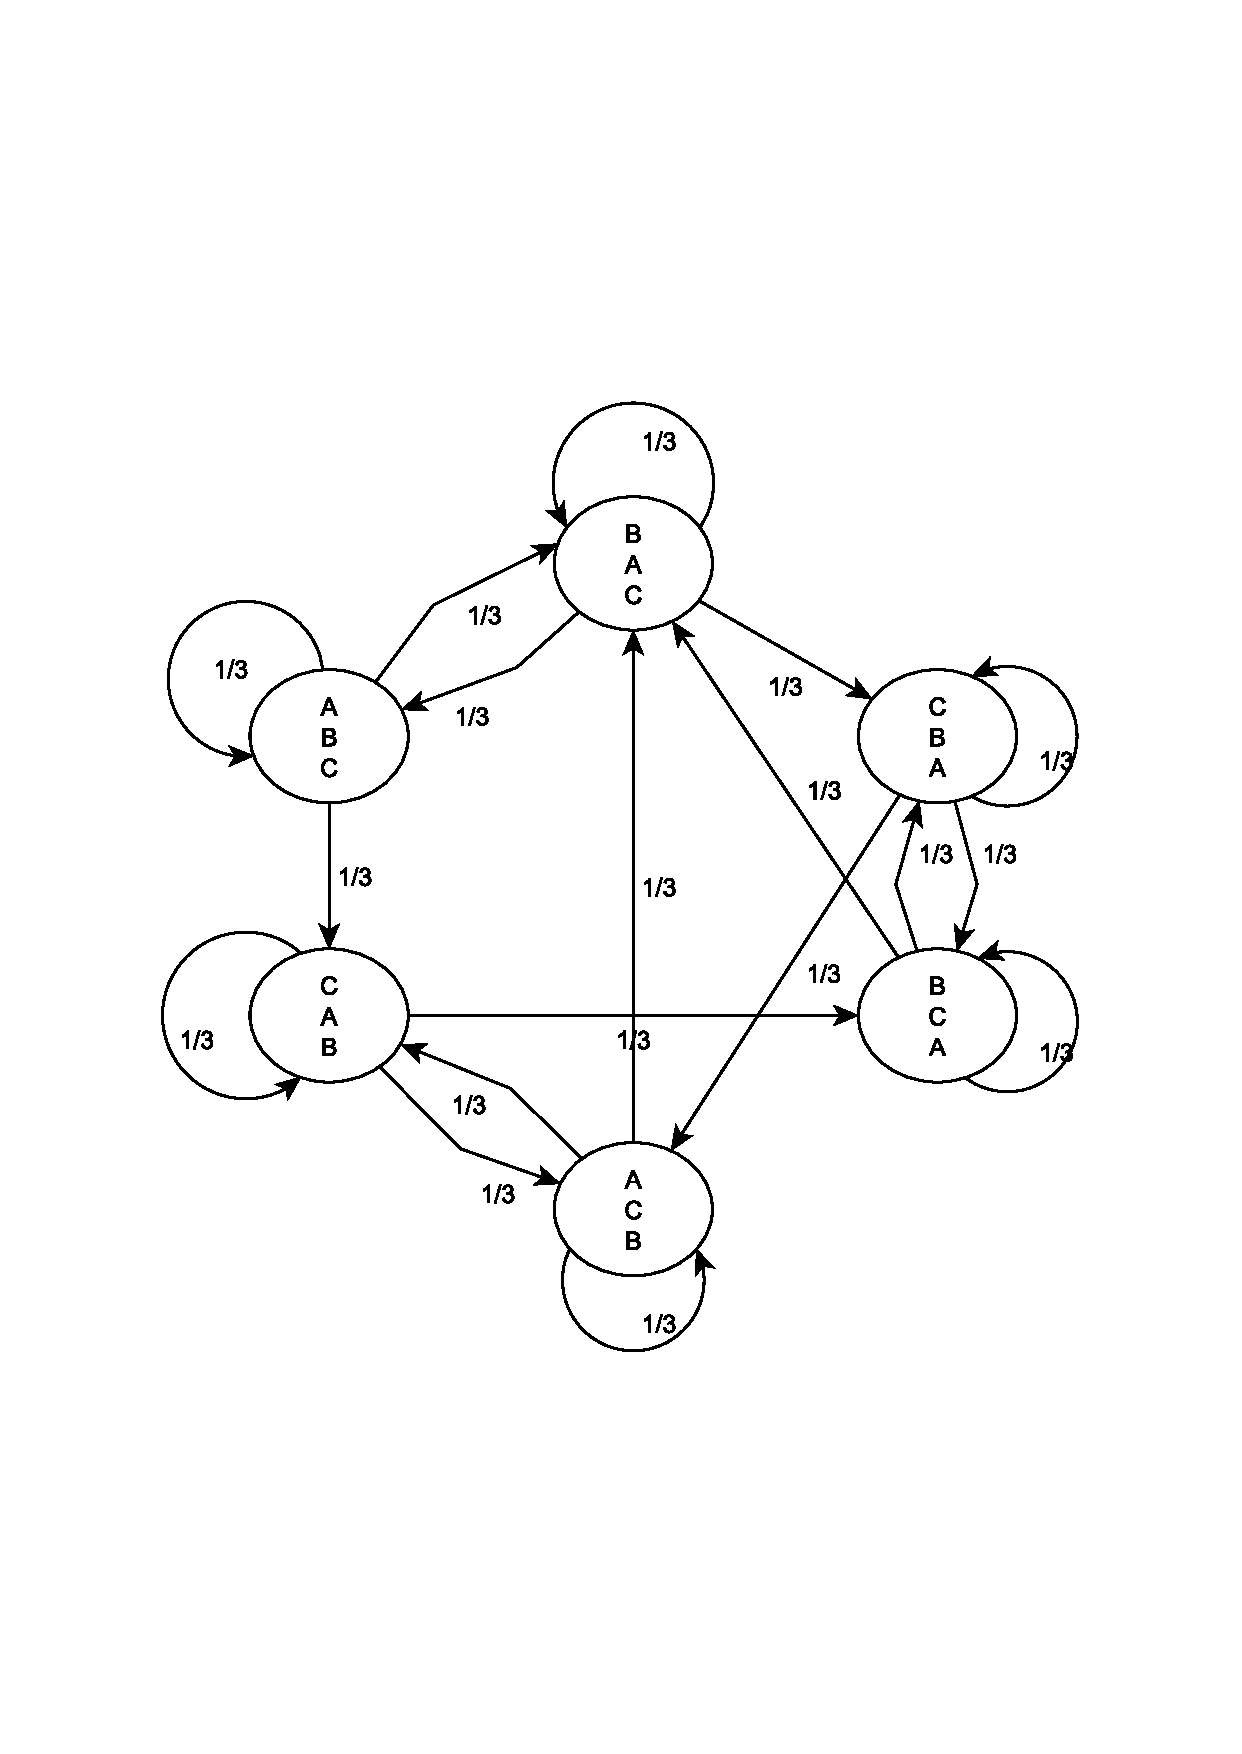
\includegraphics[scale=0.40]{cp_ex6_fig1.pdf}
\caption{Grafo delle transizioni}
\label{fig:}
\end{figure}

Dal grafo si evince che esso � fortemente connesso poich� esiste un cammino che collega ogni coppia di nodi. Risulta quindi che la catena � irrudicibile. Inoltre, essendo lo spazio degli stati finito, segue da un corollario del teorema sulle classi chiuse.

\end{document}
